\subsection{Making Counterexamples Actionable} 
We therefore desire AGREE counterexamples that are \textit{actionable}; that is, an explanation of the violation in terms that will quickly lead to a passing analysis (e.g., by making changes to the model or formal contract).
%
%In the following sections, we introduce AGREE-Dog, 
To achieve this, we implemented
an interactive conversational copilot powered by GPT-4o (omni) multi-modal generative AI, specifically developed to assist AGREE users in identifying the root causes of counterexamples and to support the subsequent model repair process. It was designed to be user-friendly and integrates with the OSATE IDE (see Figure~\ref{fig:AGREEDOG}). 
%\footnote{In Figure~\ref{fig:AGREEDOG} AGREE-Dog is a specific instance of the INSPECTA-Dog toolset, where users can select the copilot's identity. This paper focuses on the AGREE-Dog instance, while other instances of INSPECTA-Dog are beyond the scope of this discussion.}

In the remainder of this section, we detail our methodology and present our key findings using the \texttt{Integer\_Toy} and \texttt{Car} models included with the AGREE distribution.

\begin{figure*}[htbp]  
    \centering
    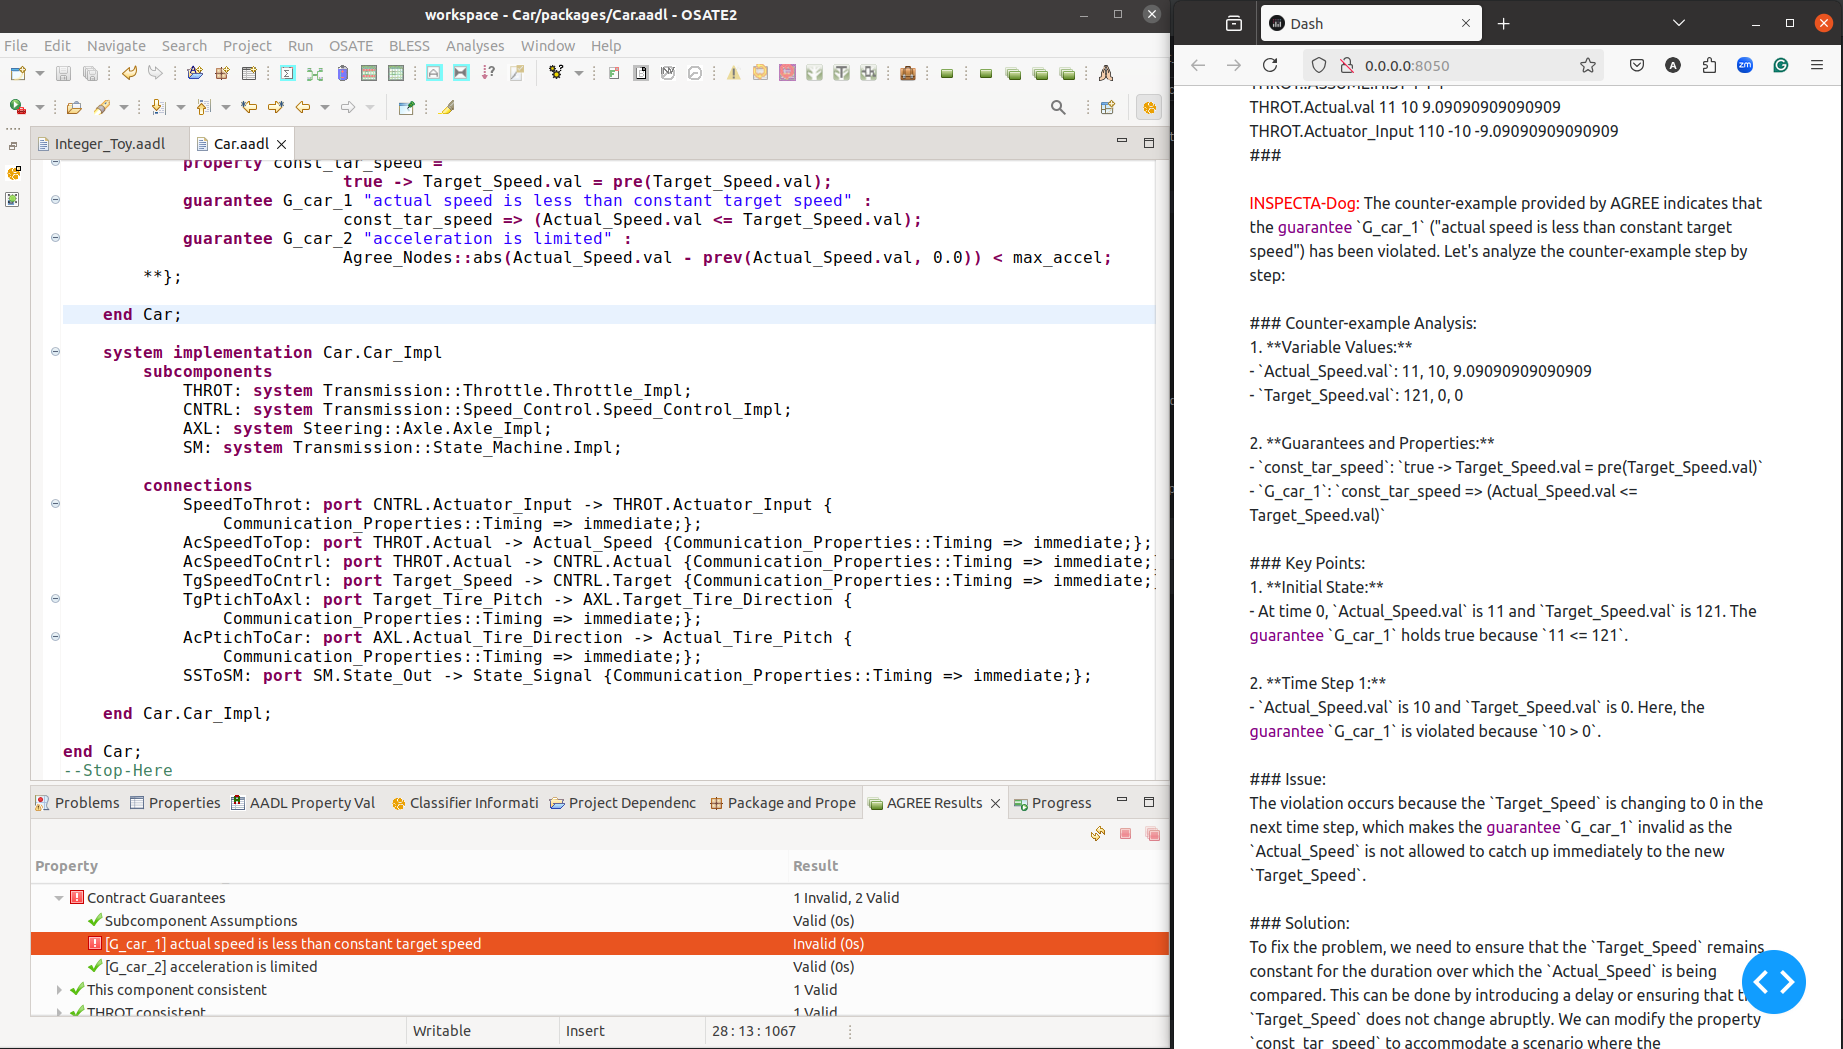
\includegraphics[width=0.9\textwidth]{AGREE-DOG-high-rs.png}%AGREE-Dog.png}  
%    \caption{AGREE-Dog, acting as a copilot to OSATE, provides explanations for the counterexample generated by the AGREE tool for the AADL model \texttt{Car.aadl}.}
    \caption{AGREE copilot in OSATE provides an explanation for a counterexample generated on the \texttt{Car} model.}
    \label{fig:AGREEDOG}
\end{figure*}


 %In the remainder of this section, we detail our methodology, for addressing the primary challenges we have encountered, present our key findings, and discuss the current limitations and directions for future work. To elucidate these challenges, we use the \texttt{Toy\_Integer} and \texttt{Car} models included with the AGREE distribution as two running examples throughout the paper.

\subsection{Contextual Prompt Constraints Problem}

The GPT-4o generative multi-modal model exhibits significant power in translating human instructions into code and vice versa, particularly when the language in question has been part of its pre-training data and there exists a substantial open-source code base, such as C or Python. However, this capability comes with the drawback of potential hallucinations. Since AGREE is not as widely adopted as languages like C or Python, this problem is exacerbated. 
%Consequently, one of the primary challenges we encountered involved the explainability of counterexamples due to the absence of relevant context.
Consequently, the lack of relevant context is a significant challenge for generating explainable AGREE counterexamples. 

%\subsubsection{AGREE-Dog Retrieval-Augmented Generation (RAG) System}
% To mitigate the Contextual Prompt Constraints problem we designed AGREE-Dog RAG system we implemented the system to be dynamic, allowing it to adjust its context based on user inquiries. 
To mitigate the contextual prompt constraints problem, we implemented a dynamic Retrieval-Augmented Generation (RAG) system, allowing it to adjust its context based on user inquiries.

Despite GPT-4o's 128k token capacity, which we estimate can accommodate several thousand lines of AADL in a single prompt, uploading an entire repository's contents can be prohibitively expensive and may well exceed the prompt token limitations. We therefore implemented a practical two-step optimization technique to meet our current needs.

First, the RAG system reads the top-level AADL file.  It then parses the file's import chain, extracting only the files in the model workspace that are specified on this chain. This step significantly reduces the initial prompt size. %, see Figure \ref{fig:AGREEDOG}.  
%
The second optimization addresses another practical requirement: handling parts of the repository that may have been included in the model's pre-training data, such as core libraries. To manage this, the RAG system applies a filtering technique to the file names, guiding the system to ignore certain files, such as standard libraries, and retain user-defined files. This approach further reduces the initial prompt size to include only files that the model has not previously encountered. Finally, user inputs are automatically incorporated into the extracted context from the current file and its import chain, allowing for more accurate responses to user inquiries.

This approach significantly mitigates contextual constraint-based hallucinations that can arise from the absence of AADL model specifications. However, it does not address the absence of the counterexample itself or the lack of guidance on the critical system requirements that should be preserved during the model repair process.
 

\subsection{Model Repair Problem}

Given that counterexamples are generated interactively and may not be included in the initial context, we dynamically extend the RAG system. This allows users to upload an exemplar AADL/AGREE model along with a corresponding counterexample (in text or CSV format). %(Figure \ref{fig:AGREEDOG2}).
Upon submission, the copilot provides a detailed, step-by-step explanation of the counterexample, identifies its root cause(s), and suggests potential solutions, as shown in Figure~\ref{fig:AGREEDOG}. 


However, a significant challenge encountered was that these explanations and suggested alternatives could include two types of hallucinations, both syntactic and semantic. The former are typically minor and can be detected and resolved using a multi-shot approach. The latter are more problematic, as the copilot might suggest altering a component's guarantee, which could successfully remove the counterexample but risk violating core system requirements that should remain unchanged.  We refer to this as the \textit{Model Repair Problem}. 


\subsubsection{Requirements for Counterexample Explanations}

To mitigate the Model Repair Problem, we configured the tool to generate solutions that conform to a predefined set of system requirements written in natural language, which are uploaded via a CSV file or directly included in the context. 

\begin{figure}[t]  
    \centering
    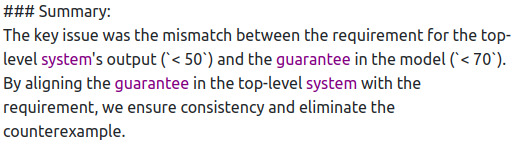
\includegraphics[width=0.95\columnwidth]{REQ-AWARE-REF-high-res.png}  
    \caption{Refined explanation using a requirements file for the \texttt{Integer\_Toy} model.}
    \label{fig:REQ-AWARE-EXPL}
\end{figure}


As a result, the tool was able to more accurately identify the root cause and suggest appropriate solutions, as demonstrated in Figure~\ref{fig:REQ-AWARE-EXPL}.
%
%For instance, in the \texttt{Toy\_Integer} model, a basic requirement like \texttt{guarantee\_3} (\texttt{certain\_variable < 50}) might suggest adding to component C. While this could eliminate the counter-example, it may not align with the intentions of the system engineers and domain experts, leading to what we consider a candidate for requirement absence hallucinations.
%
This refinement significantly enhanced the accuracy of the recommendations.


\subsection{Preliminary Results and Conversational Quality Assessment Problem}
 
Our initial evaluations were conducted manually, focusing on the copilot's ability to accurately identify the root cause of the counterexamples, repair the model, and ensure compliance with the requirements. The system was evaluated on two case studies. The first case study involved the \texttt{Integer\_Toy} model, while the second dealt with a larger model that imports several files, totaling 7 files and approximately \texttt{380} lines of AADL. The copilot successfully identified the root cause of all counterexamples for the specified guarantees (13 out of 13) on the first attempt, demonstrating a high degree of accuracy.
%
However, these manual evaluations highlight the need for greater automation; consequently, we plan to develop a more automated evaluation system to enable testing on more realistic and complex use cases.
%, following the workflow shown in Figure~\ref{fig:CQAS}.
 

%\begin{figure}[htbp]
%\centering % Still centering the figure
%\hspace*{-1cm} % Shift the entire figure to the left by 1 cm
%\resizebox{0.95\columnwidth}{!}{ % Keep the size slightly below the full column width for better fit
%\tikzstyle{root} = [rectangle, fill=white!3, text width=4.5em, text centered, minimum height=2em, node distance=.10cm]
%\tikzstyle{block} = [rectangle, draw, fill=blue!3, text width=5.3em, text centered, minimum height=2em, node distance=.40cm]
%\tikzstyle{block1} = [rectangle, draw, fill=red!3, text width=7em, text centered, minimum height=2em, node distance=.5cm]
%\tikzstyle{block2} = [rectangle, draw, fill=gray!3, text width=6em, text centered, minimum height=2em, node distance=.5cm]
%\tikzstyle{block3} = [rectangle, draw, fill=green!10, text width=8em, text centered, minimum height=2em, node distance=.55cm]
%\tikzstyle{line} = [draw, -latex']
%
%\begin{tikzpicture}[auto, node distance=2cm,>=latex']
%    % Place nodes
%    \node [root] (root1) {};
%    \node [block1, right=of root1] (interactions) {\texttt{\textbf{AGREE-Dog}} User-System Interactions};
%    \node [block2, below=of interactions] (history) {Conversation History Management};
%    \node [block2, right=of history] (lemma) {Model-Repair Multi-Shots Dictionaries};
%    \node [block2, right=of lemma] (quality) {Collecting Quality Metrics Automatically};
%    \node [block3, above=of quality] (stat) {\textcolor{blue}{Statistical Analysis and Visualization}};
%
%    % Draw edges
%    \path [line] (root1)  (interactions);
%    \path [line] (interactions) -- (history);
%    \path [line] (history) -- (lemma);
%    \path [line] (lemma) -- (quality);
%    \path [line] (quality) -- (stat);
%\end{tikzpicture}
%} % End of resizebox
%\caption{AGREE-Dog Conversation Quality Assessment System (CQAS) workflow.}
%\label{fig:CQAS}
%\end{figure}

We are in the process of selecting a golden set of examples from a formally verified library we developed previously, and constructing a testing set by introducing deliberate violations. These examples will be used by the copilot to evaluate its ability to correctly identify the root causes. While we have demonstrated initial success in this area, model repair remains a more complex challenge. This is because repairing models can result in multiple solutions, particularly for more intricate use cases. One of the key limitations is the tool's ability to consistently remove counterexamples while ensuring compliance with the specified requirements. To address these issues, we are developing a toolset aimed at measuring convergence towards the correct semantics of the golden examples, within a few-shot learning context. This remains an ongoing challenge that we will address in our future work. %extend our prior research from the \cite{coqDog} paper to improve AGREE-Dog's performance in these areas


%\subsection{Preliminary Results}
